\documentclass[11pt,a4paper]{article}
\usepackage[T1]{fontenc}
\usepackage[utf8]{inputenc}
\usepackage[brazil]{babel}
\usepackage{lmodern}
\usepackage[margin=2.5cm]{geometry}
\usepackage{graphicx,float,xcolor}
\usepackage[hidelinks]{hyperref}
\usepackage{microtype}
\setlength{\parskip}{0.6em}
\setlength{\parindent}{0pt}
\graphicspath{{../notebooks/figs/}}
\newcommand{\campo}[1]{\texttt{#1}}
\newcommand{\onde}{\textbf{Onde aparece.} }
\newcommand{\problema}{\textbf{Por que é um problema.} }
\newcommand{\decisao}[1]{\textbf{Decisão: #1.} }

\title{\textbf{Relatório de limpeza e preparação dos dados}\\[0.3em]\large Projeto Extensionista: análise de dados de enchentes do INCT SiMAI\\Coleta, Preparação e Análise de Dados (Fase 2)}
\author{Autor: João Pedro da Silva Kriger}
\date{10 de novembro de 2026 (revisado em 25 de novembro de 2026)}

\begin{document}
\maketitle

\section{O que o projeto quer mostrar}

O dashboard tem duas telas. A \textbf{Tela 1} responde à pergunta do enunciado: se o Guaíba chegar a X metros, quais bairros e quantas pessoas são afetados. Ela usa somente o arquivo \campo{data.json} do INCT SiMAI, depois de limpo.

A \textbf{Tela 2} mostra para onde vai a verba da reconstrução de Porto Alegre. O elemento central é um slider do nível do rio: conforme a água avança, segundo a mancha simulada pelo próprio INCT, a tela mostra quais obras de reconstrução ficam na área alcançada e quanto investimento fica exposto, ou seja, o valor previsto para essas obras. Ela também compara o que a Prefeitura estima precisar com o que foi solicitado e recebido. A ligação com a Tela 1 é o mesmo nível do rio e a mesma simulação.

Este relatório descreve, para cada base, os problemas encontrados e o que foi decidido. A seção~\ref{sec:inct} trata do \campo{data.json}; as seções~\ref{sec:manchas} a \ref{sec:slider}, das bases da Tela 2; a seção~\ref{sec:escopo}, das análises exploradas na concepção do projeto e cortadas do escopo.

\section{Bases utilizadas}

\textbf{Simulação do INCT SiMAI.} O \campo{data.json}, fornecido pela disciplina, e as manchas simuladas de cada nível de 3,0 a 5,4 m, obtidas da mesma API usada pelo site do INCT em 10/11/2026.

\textbf{Prefeitura de Porto Alegre (servidor ArcGIS, coletado em 27/10/2026).} A malha dos 94 bairros e as cotas de inundação; as obras do painel Monitoramento da Reconstrução, com tipo, local, valor previsto e situação; as etapas e contratos das obras do sistema de proteção; as áreas de habitação do DEMHAB; e os valores de necessidade, solicitado e recebido do painel financeiro.

\textbf{TCE-RS (dados abertos, coletados em 27/10/2026).} Contratos, licitações e empenhos de 2024 e 2025 da Prefeitura e do DMAE. Usados só para conferir os valores das obras do DMAE (seção~\ref{sec:obras}).

\textbf{Copernicus EMSN194 (União Europeia, coletado em 04/11/2026).} Os pontos do produto P08, com os prédios atingidos em 2024.

\section{O arquivo da simulação (\texttt{data.json})}
\label{sec:inct}

O arquivo tem 71 níveis do rio, de 3,0 a 10,0 m, e 94 bairros, ou seja, 6.674 registros. Cada registro traz o total de prédios do bairro, os prédios afetados, a porcentagem de prédios afetados, a população do bairro e a população afetada estimada. Nenhum valor original foi apagado: o arquivo limpo guarda os originais em colunas próprias, e cada alteração de prédios afetados está registrada em \campo{inct\_alteracoes.csv}.

\subsection{Como o arquivo foi testado}

O ponto de partida foi uma ideia simples: se a simulação está coerente, certas regras precisam valer em todos os registros. Foram testadas dez regras sobre o arquivo original. O documento \campo{relatorios/provas\_testes\_inct.pdf} demonstra os testes de conteúdo com gráficos ou quadros.

Cinco testes passaram. Todos os 71 níveis têm os mesmos 94 bairros, sem falta nem repetição, e os nomes são escritos do mesmo jeito em todos os níveis. Não há valor nulo nem negativo. O total de prédios e a população de cada bairro são iguais em todos os níveis. Os prédios afetados nunca passam do total do bairro; em 336 registros os dois são iguais, o que indica bairro totalmente atingido.

Os outros cinco revelaram problemas: a ordem dos bairros muda em 5,3 m; a porcentagem não corresponde à conta exata em 2.620 registros; a população afetada herda esse erro; em 12 momentos os prédios afetados de um bairro diminuem quando o rio sobe; e a população afetada na cidade cai uma vez, entre 9,6 e 9,7 m.

\subsection{Inconsistências e tratamento}

\textbf{1. Porcentagem arredondada sempre para cima.} \onde Em 6.672 dos 6.674 registros, \campo{percentage} é a porcentagem real arredondada para cima. No Cristal, a 3,0 m, são 20 de 10.229 prédios (0,20\%), e o arquivo informa 1\%. A diferença passa de 0,01 ponto em 2.620 registros; nos demais, a porcentagem real já é inteira ou quase, como nos 3.693 registros com 0\% e nos 336 com 100\%. As duas exceções são de Boa Vista do Sul, a 7,2 e 7,3 m: 686 de 2.450 prédios dá exatamente 28\%, e o arquivo traz 29\%, efeito típico de erro de arredondamento do computador. \problema O enunciado diz que o campo é calculado a partir dos prédios, e o resultado fica sempre acima do real, com erro maior onde poucos prédios foram atingidos. O enunciado não diz como arredondar, então pode ter sido uma escolha do INCT. \decisao{corrigir} O campo foi recalculado como prédios afetados divididos pelo total, vezes 100, com duas casas. O valor antigo fica em \campo{percentage\_original}.

\textbf{2. População afetada inflada.} \onde \campo{affected\_population} é a população multiplicada pela porcentagem arredondada, arredondada de novo para cima. No Cristal, o arquivo informa 249 pessoas, e a conta exata dá 49. \problema Somando a cidade, o excesso fica entre 1.328 e 3.963 pessoas conforme o nível: 4,8\% do valor exato a 3,0 m e 1,5\% a 5,3 m. Em bairros com poucos prédios atingidos a distorção é grande: em Petrópolis, a 7,1 m, um único prédio atingido vira 377 pessoas. \decisao{corrigir} O campo foi recalculado com a porcentagem exata. O resultado continua sendo estimativa, porque supõe a população distribuída igualmente entre os prédios.

\begin{figure}[H]\centering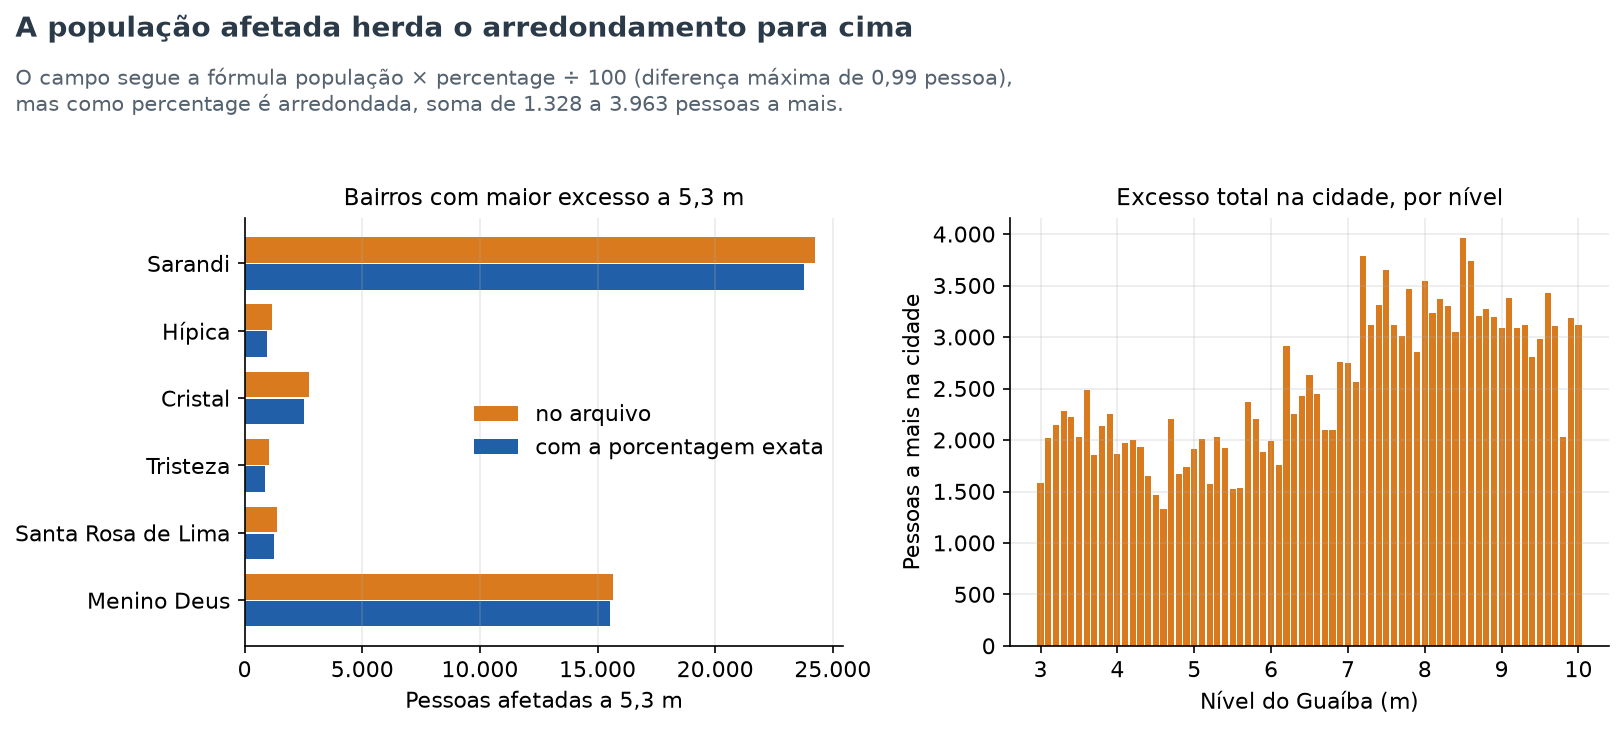
\includegraphics[width=0.88\textwidth]{prova_t6_populacao.png}\caption{Excesso de população causado pelo arredondamento.}\end{figure}

\textbf{3. Zeros no meio da série.} \onde No Centro Histórico, a contagem vai de 2.050 prédios em 9,6 m para zero em 9,7 e 9,8 m e volta a 2.130 em 9,9 m. No Rubem Berta, o zero está em 8,8 m, entre 252 e 285. No Lageado, em 8,1 m, entre 108 e 110. \problema Era esperado que a contagem só subisse ou ficasse igual, já que cada nível parece usar o mesmo método. O zero do Centro Histórico derruba a população afetada da cidade de 264.338 para 252.080 em 9,7 m. \decisao{interpolar} Cada zero foi trocado por uma reta entre os vizinhos válidos: 2.077 e 2.103 no Centro Histórico, 269 no Rubem Berta e 109 no Lageado. A série é suave dos dois lados.

\textbf{4. Bloco inicial no Espírito Santo.} \onde De 3,0 a 3,3 m são 637 prédios afetados, e em 3,4 m, 633. Em 3,5 m o valor cai para 25, e a série só chega a 133 em 10,0 m. \problema Cinco níveis baixos com mais prédios do que qualquer nível alto. \decisao{corrigir, com ressalva} Os cinco níveis recebem 25, o primeiro valor plausível e o maior compatível com a regra de não diminuir. O valor verdadeiro é desconhecido.

\textbf{5. Pico isolado no Espírito Santo.} \onde 2.101 prédios em 4,7 m, entre 46 e 47 nos vizinhos. \problema Um salto de um único nível acrescenta mais de 2 mil prédios ao total da cidade. \decisao{interpolar} O valor foi substituído por 46.

\textbf{6. Oscilações no Arquipélago.} \onde O bairro varia entre 4.674 e 4.688 prédios, com seis quedas de no máximo 11 prédios. A série fica em 4.680 e sobe para 4.685 exatamente em 3,0, 3,5, 4,0, 4,5 e 5,0 m, e para 4.688 em 5,3 m, o que pode indicar níveis gerados separadamente. \problema As quedas contrariam a regra, mas representam no máximo 0,3\% do bairro. \decisao{corrigir com ajuste mínimo} Cada nível recebe o maior valor visto até ali, o que altera 65 valores sem efeito perceptível no total.

\begin{figure}[H]\centering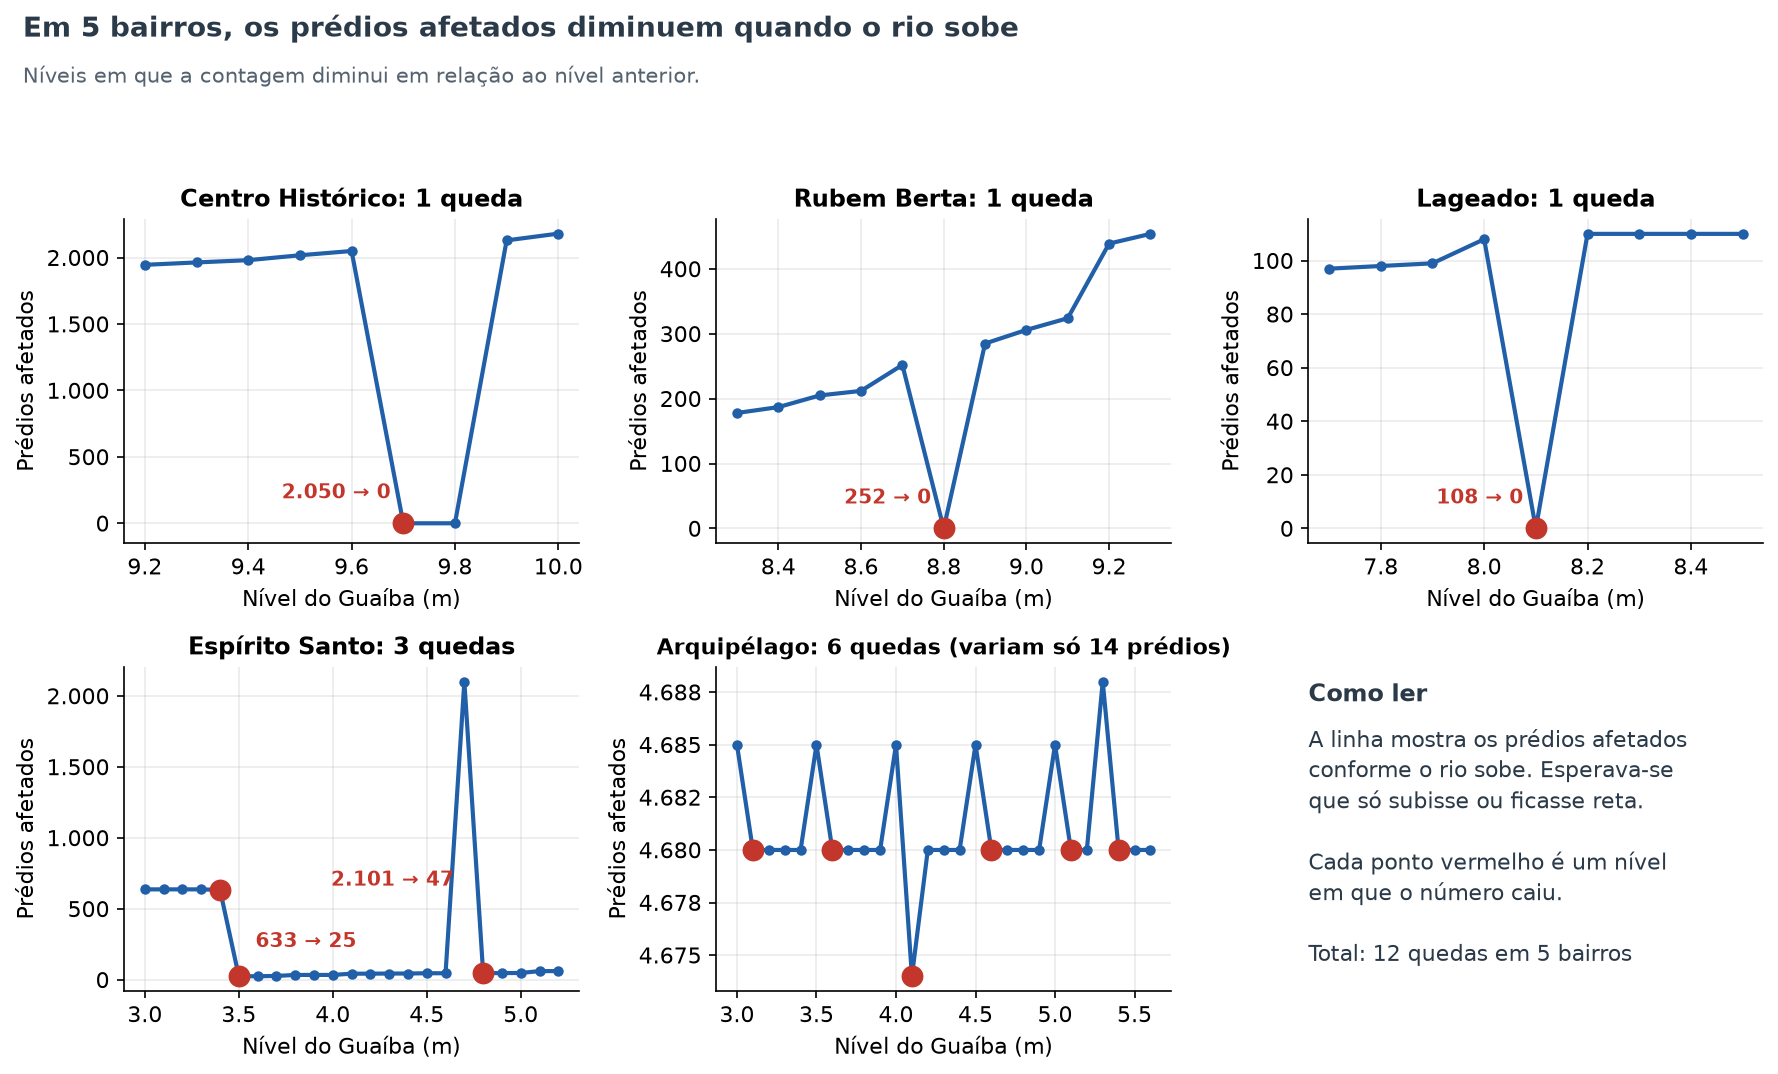
\includegraphics[width=\textwidth]{prova_t7_quedas.png}\caption{Os cinco bairros em que os prédios afetados diminuem quando o rio sobe.}\end{figure}

\textbf{7. Bairro fora de ordem.} \onde Em 5,3 m, Morro Santana sai da 57ª posição e vai para a última, deslocando 38 bairros. \problema Quem lê o arquivo pela posição mistura bairros; a mudança também sugere geração separada desse nível. \decisao{corrigir} O arquivo limpo é ordenado por nível e bairro, e todo acesso é feito pelo nome. Nenhum valor muda.

\textbf{8. Nomes diferentes da malha oficial.} \onde Coronel Aparício Borges aparece como Aparício Borges na malha da Prefeitura, e Mont'Serrat como Montserrat. \problema Na junção pelo nome, esses bairros ficariam sem cor no mapa. Nenhum dos dois é atingido. \decisao{manter e mapear} A coluna \campo{bairro} preserva o nome do INCT, e \campo{bairro\_malha} traz o oficial. O script confere a correspondência dos 94 bairros.

\textbf{9. Limitações da simulação.} \onde A população é distribuída igualmente entre todos os prédios, inclusive os não residenciais; 40 bairros nunca são atingidos; e há 210 registros com apenas 1 a 19 prédios afetados. \problema Não são erros do arquivo, mas limitam a interpretação. \decisao{manter e avisar} O aviso de limitações da Tela 1 explica isso.

\subsection{Em que faixa do rio estão os erros}

A enchente de 2024 chegou a 5,35 m. Até esse nível, os valores correspondem a alturas que o rio já atingiu; acima, são cenários hipotéticos. Das 12 quedas, 8 estão até 5,3 m: três do Espírito Santo e cinco do Arquipélago. As outras 4 estão acima do recorde, incluindo todos os zeros isolados. Por isso o Espírito Santo é o caso mais importante: está na faixa mais realista, e o valor correto é desconhecido. Os erros acima do recorde também foram corrigidos, porque a Tela 1 mostra todos os níveis até 10,0 m, e o aviso informa que esses níveis são hipotéticos.

\subsection{Efeito da limpeza e verificação}

Foram alterados 75 valores de prédios afetados, em 5 bairros, e a porcentagem e a população foram recalculadas em todos os registros. A 3,0 m, a estimativa cai de 34.605 para 32.119 pessoas, e os prédios, de 15.264 para 14.652. A 4,7 m, as pessoas passam de 120.271 para 115.027, e os prédios, de 47.521 para 45.471. A 5,3 m, os prédios ficam em 53.989 e as pessoas caem de 138.414 para 136.389. A 9,7 m, as pessoas sobem de 252.080 para 263.710. A 10,0 m, passam de 274.993 para 271.886.

\begin{figure}[H]\centering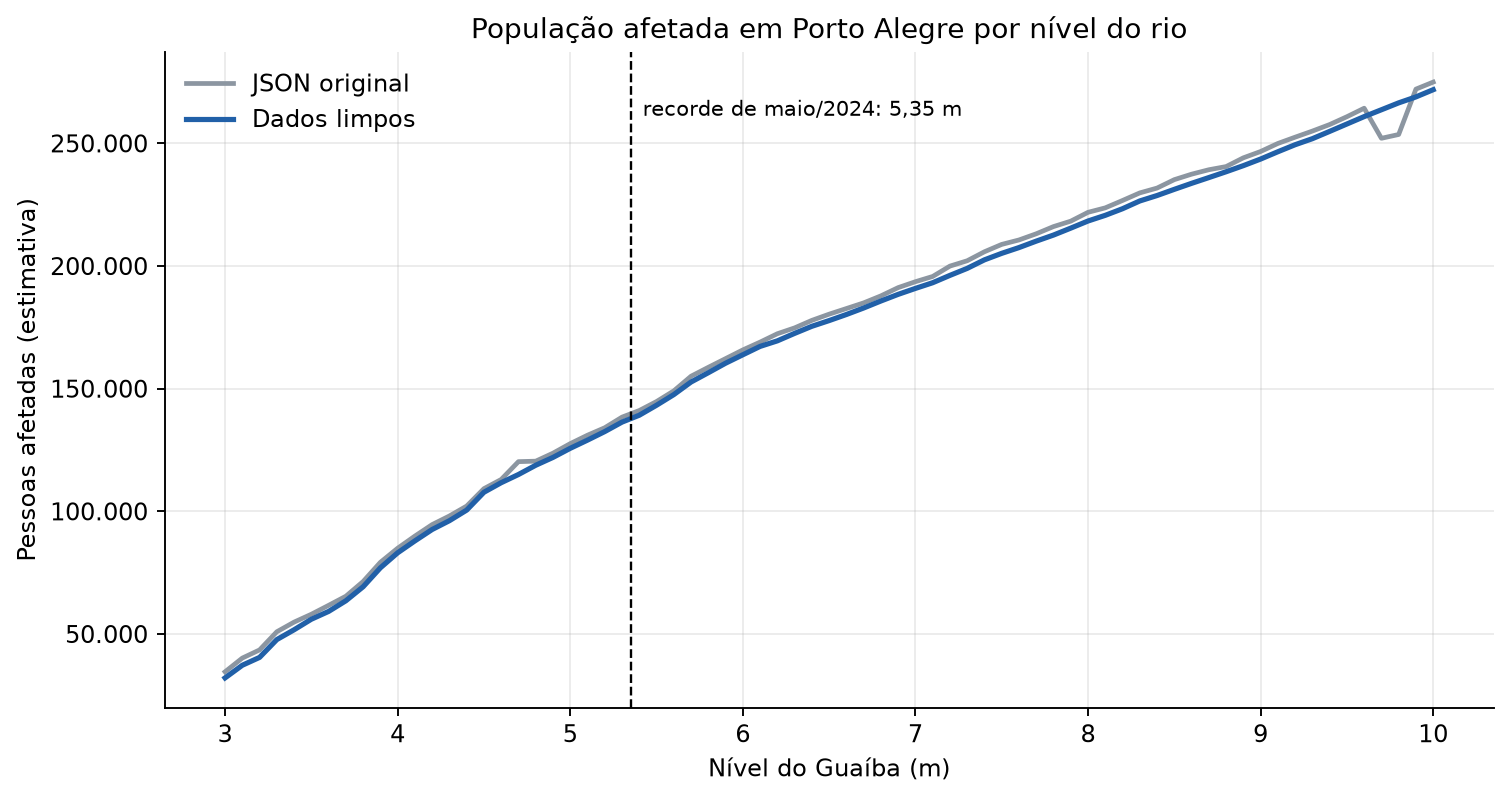
\includegraphics[width=0.78\textwidth]{g1_curva_populacao.png}\caption{População afetada por nível: a queda em 9,7 m desaparece após a limpeza.}\end{figure}

Depois da limpeza, o script confere automaticamente que há 71 níveis com 94 bairros, que os prédios afetados nunca caem, que a porcentagem fica entre 0 e 100, que os prédios afetados não passam do total, que a curva de população só sobe e que todos os bairros existem na malha oficial. Todas as verificações passaram.

\section{Manchas do INCT por nível}
\label{sec:manchas}

\textbf{O que são.} A mancha é o polígono da área que a simulação do INCT indica como alagada em um nível do Guaíba, o mesmo desenho azul que aparece no site do INCT. Ela cobre a terra alagada e também rios e canais, como o Jacuí e o Gravataí, mas não cobre o lago Guaíba aberto, e termina num retângulo, que é o limite da área simulada. É ela que diz até onde a água chega na Tela 2.

\textbf{Como foram obtidas.} O site do INCT busca cada mancha numa API (\campo{POST http://vhlab.lad.pucrs.br:5002/api/map-data}). O script \campo{scripts/coleta\_bases.py --temas inct} faz a mesma consulta que o site, uma por nível: o nível vai no campo \campo{water\_level}, e os filtros de bairro, rua e endereço vão vazios, para que a resposta traga a mancha inteira. Há pausa de 5 segundos entre as consultas. Foram baixados os 25 níveis de 3,0 a 5,4 m, em 10/11/2026, e cada resposta foi guardada sem alteração em \campo{dados/originais/1\_simulacao\_inct/mancha\_inct\_api/}, num arquivo por nível (\campo{map\_data\_3\_0m.json}, \campo{map\_data\_3\_1m.json} e assim por diante). A mancha está na chave \campo{flood} da resposta, como um único multipolígono em latitude e longitude; as demais chaves descrevem o estilo e a posição do mapa no site e não são usadas.

\textbf{Como foram preparadas.} A mesma preparação é feita em \campo{scripts/obras\_por\_nivel.py}, que faz as contas, e em \campo{scripts/prepara\_dashboard.py}, que gera os arquivos do app. Para cada nível, o script lê o multipolígono da chave \campo{flood}; converte as coordenadas para o sistema SIRGAS 2000 / UTM 22S (EPSG:31982), que é em metros, para que distâncias e áreas possam ser medidas; corrige as partes do desenho que se cruzam ou têm defeito de geometria (função \campo{make\_valid}); e junta todas as partes numa só geometria. A mancha não é recortada pelo limite do município: ela já não cobre o lago, e o limite simplificado dos bairros cortaria faixas de orla onde ficam obras.

Para as contas, a mancha é alargada em 50 m para todos os lados, e uma obra conta como alcançada quando o seu ponto cai dentro dessa faixa (seção~\ref{sec:slider}). Para o mapa do app, o desenho é simplificado com tolerância de 15 m, só para carregar mais rápido, e gravado em \campo{dados/processados/dashboard/manchas/}, um GeoJSON por nível. As contas sempre usam a mancha original, e não a simplificada.

\textbf{Papel da malha de bairros.} A malha oficial de bairros não corta a mancha. Ela serve para montar o contorno do município, que é usado para medir a área da mancha dentro de Porto Alegre e para separar os pontos do Copernicus que ficam na cidade. Como a malha é uma versão simplificada, os bairros vizinhos não se encaixam perfeitamente e sobram frestas entre eles; por isso o contorno é montado juntando os 94 bairros e usando só a borda externa de cada parte, o que fecha essas frestas. A malha também é usada para comparar a mancha com o \campo{data.json} bairro a bairro.

\textbf{Conferências.} A área da mancha dentro do município cresce a cada nível, de 88 km² a 3,0 m para 138 km² a 5,4 m, e o script para com erro se ela diminuir. A mancha também é coerente com o \campo{data.json}: a 3,0 m, os bairros com mais de 1\% da área dentro da mancha são exatamente os 24 que o arquivo dá como atingidos (outros 4 só encostam na mancha), e a 5,3 m a parcela da área de cada bairro coberta pela mancha acompanha a porcentagem de prédios atingidos (correlação de 0,97).

\section{Obras e verba da reconstrução}
\label{sec:obras}

\textbf{Obras do painel da Prefeitura.} O local e o tipo das obras são confiáveis: as coordenadas caem no bairro informado em quase todos os casos. Os valores, não. São investimentos previstos, e não valores enviados ou pagos. Dos 293 valores, 112 (38\%) se repetem três vezes ou mais, sinal de rateio ou valor-padrão. Para conferir, os valores das obras do DMAE foram comparados com os contratos do TCE-RS, pela empresa e pelo valor de contrato que a Prefeitura informa (\campo{scripts/cruza\_obras\_contratos.py}): em três casos, o valor de cada obra é um contrato dividido em partes iguais entre vários projetos, o que confirma o rateio. Esse é o único uso do TCE-RS no projeto. O valor do mesmo projeto difere entre camadas em 109 de 114 casos. A situação da obra falta em cerca de metade dos pontos do sistema de proteção e conflita entre camadas em 12 projetos. A data de atualização é a mesma em todos os registros, 17/09/2026, que é a data da exportação. Por isso os valores aparecem sempre como ``previstos'' e só como ordem de grandeza. O detalhamento está em \campo{dados/processados/auditoria\_base\_reconstrucao.md}.

\textbf{Habitação (DEMHAB).} O valor é um custo estimado de reposição, e só 34 das 120 áreas seguem a regra de multiplicar os domicílios inabitáveis por R\$ 170 mil. Ele aparece como necessidade estimada, separado das obras.

\textbf{Painel financeiro.} A Prefeitura estima em R\$ 12,3 bilhões o prejuízo da enchente ao setor público, valor que a Prefeitura apresentou ao governo federal por ofício como estimativa de prejuízo. Esse valor inclui R\$ 5,5 bi em habitação, R\$ 4,7 bi em expansão da macrodrenagem e R\$ 602,8 mi em perda de arrecadação. O painel registra R\$ 164,4 mi recebidos de R\$ 182,8 mi solicitados para emergência e R\$ 8,4 mi de R\$ 196,6 mi para reconstrução. A camada não diz quem repassa, mas o texto do painel confirma que os pedidos foram feitos à União por cadastros formais do governo federal, como os da Defesa Civil e do Ministério da Saúde, num total de R\$ 381,9 milhões; nos dados, o total solicitado é de R\$ 379,4 milhões.

\textbf{Comparação com o painel oficial.} Em 10/11/2026, os números do site do painel foram comparados com os dados abertos que ele publica, com registros de 17/09/2026. Parte confere, como os R\$ 620,6 milhões do sistema de proteção; outra parte não, como as obras de infraestrutura, que no site são 219 e nos dados, 194. Por isso, o dashboard informa a fonte e a data dos dados.

\textbf{Copernicus P08.} Marca prédios e instalações atingidos por interpretação visual de imagens de 0,5 m. Em Porto Alegre são 42,6 mil marcações, das quais 1.930 de dano possível e 789 de instalações industriais. Cobre só parte da cidade e não foi conferido em campo, por isso entra no mapa apenas como camada de locais atingidos.

\section{Como o slider da Tela 2 é calculado}
\label{sec:slider}

\textbf{Ideia.} O slider responde a uma pergunta: com o rio a um certo nível, quais obras de reconstrução ficam na área que a água alcança, e quanto de investimento está previsto nelas? Esse valor é chamado aqui de \textbf{investimento exposto}. Ele não é uma previsão de custo de dano: o valor de cada obra é o que a Prefeitura prevê gastar para reconstruir ou reforçar o que foi atingido em 2024, e não quanto custaria repará-la se fosse atingida de novo. Além disso, as obras do sistema de proteção existem justamente para segurar a água, e o valor delas não vira dano se funcionarem. O investimento exposto mostra quanto da verba da reconstrução está indo para lugares que a água alcança. A resposta é obtida obra por obra, a partir da localização de cada uma, e não por aproximação de bairro. Uma conta por bairro, como multiplicar a porcentagem atingida do bairro pela verba do bairro, suporia que as obras estão espalhadas por igual dentro dele, o que não é verdade: uma escola na parte alta de um bairro parcialmente atingido seria contada como atingida.

\textbf{Passo a passo.} O script \campo{scripts/obras\_por\_nivel.py} faz quatro etapas para cada nível de 3,0 a 5,4 m, em passos de 0,1 m:
\begin{enumerate}
\item transforma cada obra em um ponto no mapa, usando os campos \campo{latitude} e \campo{longitude} da base de reconstrução da Prefeitura;
\item lê a mancha do INCT daquele nível, inteira e preparada como descrito na seção~\ref{sec:manchas};
\item testa, para cada ponto, se ele está dentro da mancha ou a até 50 m dela;
\item conta as obras que passaram no teste e soma o investimento previsto delas, que é o investimento exposto naquele nível, separando sistema de proteção e equipamentos públicos.
\end{enumerate}
Todas as contas de distância são feitas em metros, no sistema SIRGAS 2000 / UTM 22S (EPSG:31982). O resultado fica no arquivo \campo{obras\_por\_nivel.csv}, em \campo{dados/processados/}, uma linha por nível.

\textbf{Quais obras entram.} Das 318 obras da base (R\$ 751,7 mi previstos), entram as 274 que têm coordenada (R\$ 740,3 mi). As 44 sem coordenada ficam de fora; 43 delas são do DMAE, quase todas prédios de apoio de estações e casas de bombas. As coordenadas existentes são confiáveis: 267 das 274 caem no bairro informado.

\textbf{Resultado.} Com o rio a 3,0 m, já são 129 obras e R\$ 447,1 mi de investimento exposto; a 4,0 m, 224 obras e R\$ 694,8 mi; a 5,4 m, 256 obras e R\$ 713,3 mi. As obras do DMAE dominam o valor por ficarem na beira do rio. O dado mais relevante são os equipamentos públicos, como escolas, praças e unidades de saúde: já a 3,0 m, uma cheia bem menor que a de 2024, 90 deles estão na área alcançada, com R\$ 80,0 mi de investimento exposto.

\begin{figure}[H]\centering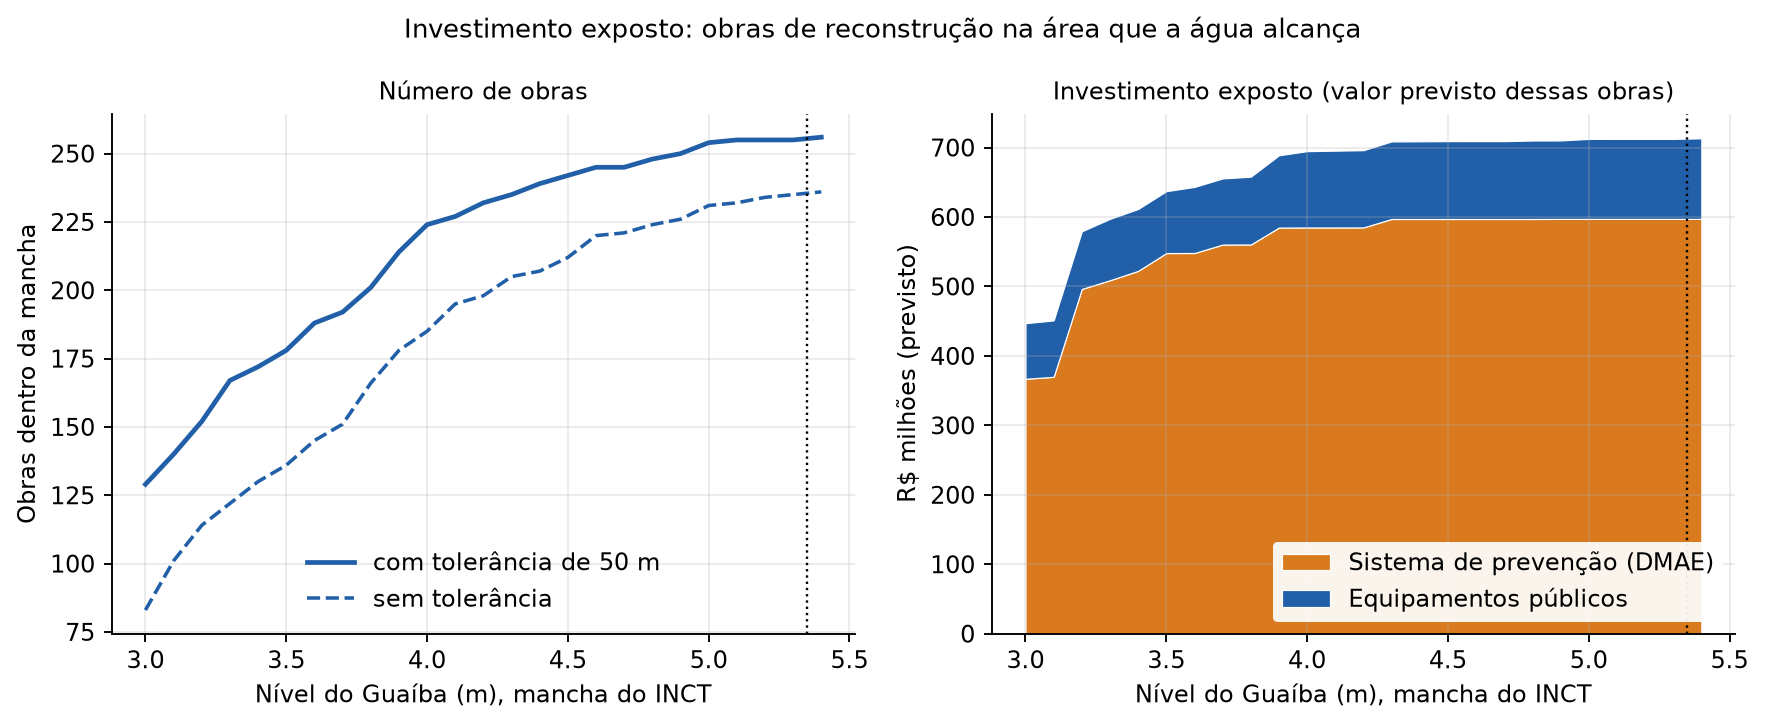
\includegraphics[width=0.95\textwidth]{g9_obras_por_nivel.png}\caption{Obras e investimento exposto dentro da mancha do INCT, nível a nível.}\end{figure}

\textbf{Limites.} O valor é previsto, não enviado nem pago. Cada obra é representada por um único ponto: isso funciona bem para uma escola ou uma praça, mas um dique de vários quilômetros fica representado por um só lugar da estrutura. A tolerância de 50 m existe para compensar isso e o desenho simplificado da mancha, mas ela muda o resultado: sem tolerância, são 83 obras a 3,0 m, e não 129, e 236 a 5,4 m, e não 256. As 44 obras sem coordenada não aparecem no slider. A mancha é simulada, e não a enchente real. O slider vai só até 5,4 m porque acima do recorde não há evento real, e o resultado praticamente não muda. Quando a Tela 1 estiver acima de 5,4 m, a Tela 2 mostra o valor de 5,4 m com um aviso.

\section{Análises cortadas do escopo}
\label{sec:escopo}

No início do projeto, na fase de concepção (\emph{inception}), antes de fechar a pergunta da Tela 2, outras análises foram exploradas. Elas foram cortadas do escopo e não fazem parte do dashboard nem de nenhum número deste relatório, e os dados delas foram apagados. Ficam registradas aqui só para mostrar o que foi considerado e por que saiu.

\textbf{Validação da mancha do INCT.} A simulação seria comparada com a mancha observada do IPH/UFRGS, com o Copernicus e com os domicílios do Censo. Saiu porque não existe uma fonte da verdade para a extensão da enchente, e a comparação viraria uma discussão de metodologia entre trabalhos de outras equipes. Ficaram só os pontos P08 do Copernicus, como registro de locais atingidos.

\textbf{Falhas do sistema de proteção.} Cronologia da cheia, áreas das casas de bombas e nível do rio pela ANA. Saiu para manter o foco na verba da reconstrução; da base de prevenção ficou só a camada de obras.

\textbf{Saúde e fila do SUS (GERCON).} Saiu porque a fila só tinha consultas com especialista, sem cirurgias, e não respondia à pergunta.

\textbf{Pontos de atenção em contratos.} Empresas sancionadas, CNPJ e licitações do Dados Abertos POA. Saiu quando a busca de pontos de atenção em contratos deixou de ser o foco; a licitação da Prefeitura também não tinha fornecedor em nenhuma das 130.506 linhas.

\textbf{Total pago com a enchente.} Os empenhos do TCE-RS mostrariam o dinheiro de fato pago. Saiu porque nenhum campo identifica toda a despesa da enchente, e um filtro por palavras no histórico erra para mais e para menos.

\section{Coleta responsável e ética}

Os arquivos \campo{robots.txt} foram verificados. O TCE-RS e o Dados Abertos POA proíbem o caminho \campo{/api/} e pedem 10 segundos entre acessos; por isso o script de coleta usa só URLs diretas de download, com essa pausa. O Copernicus proíbe \campo{/download/}, por isso os pontos P08 foram baixados manualmente. A API do INCT e o servidor da Prefeitura não têm \campo{robots.txt}, e o script faz pausas mesmo assim.

Os arquivos do TCE-RS contêm CPF e nome de credores pessoa física e não são versionados no repositório; o script os baixa. O recorte exploratório de empenhos (\campo{empenhos\_enchente.csv}) não é usado nas telas e ainda tem nomes de servidores no histórico, por isso precisa ser mascarado ou removido antes da publicação. O dashboard não publica nomes de pessoas físicas, e sinais de atenção em contratos não são tratados como prova de irregularidade.

\section{Uso de ferramenta de IA}

Utilizei o assistente Claude Code (Anthropic) entre 27/10 e 10/11/2026, e na revisão de 25/11/2026, na coleta das bases, na escrita dos scripts de limpeza e de análise, na identificação das inconsistências, no notebook, no wireframe, na redação deste relatório e na revisão dos números. As decisões e as conclusões são minhas, e conferi os resultados.

\section{Reprodução}

O processamento é reprodutível com os comandos abaixo; o notebook de análise é \campo{eda.ipynb}, na pasta \campo{notebooks/}, e o JSON limpo em formato longo é o arquivo \campo{inct\_longo\_limpo.json}, em \campo{dados/processados/}.

\begin{verbatim}
python3 -m venv .venv && .venv/bin/pip install -r requirements.txt
.venv/bin/python scripts/coleta_bases.py
.venv/bin/python scripts/limpeza_inct.py
.venv/bin/python scripts/obras_por_nivel.py
.venv/bin/python scripts/cruza_obras_contratos.py
.venv/bin/python scripts/prova_testes_inct.py
.venv/bin/python scripts/gera_wireframe.py
\end{verbatim}

\end{document}
